\subsection{Funkcinis-reaktyvus programavimas}

\subsubsection{Įvadas}

Pagrindinė funkcinio programavimo abstrakcija yra funkcija, kuri priima tam tikrą įvestį, o jos rezultatas yra tam tikrą išvestis. Funkcijos įvestis bei rezultatas gali būti kita funkcija. Funkcinėje programavimo kalboje funkcijos yra pirmos eilės reikšmės.

Priešingai, labiau populiarus imperatyvaus programavimo modelis priima sakinius arba veiksmus kaip pirminius programos konstravimo blokus, kurie modifikuoja būseną. Tokios programos turi nuoseklų kontrolės srautą ir reikalauja samprotavimo apie pašalinius efektus. Iš prigimties jie yra atsparūs kompoziciniam samprotavimui.

Netgi funkcinėse programavimo kalbose, reaktyvios programos yra paprastai parašytos imperatyviu stiliumi, naudojant žemo lygio bei ne paruoštų komponentų abstrakcijas įskaitant atgalinius skambintojus arba objektu paremtais įvykių dorokliais. Tai pririša modelį prie interaktyvumo prie žemo lygio realizacijos detalių tokių kaip laikas bei įvykių apdorojimo modeliai.

Anot \cite{Survey}, funkcinis reaktyvus programavimas, toliau vadinamas tiesiog FRP reiškia, jog modelis turi išlaikyti funkcinio protamavimo charakteristikas (pavyzdžiui, primityvios kalbos konstrukcijos turi likti pirmosios klasės) įtraukiant reaktyvumą į kalbos modelį. Funkcinis-reaktyvus programavimas yra būdas modeliuoti reaktyvų - besikeičiančius laiko tekmėje bei reaguojančius į išorinį stimulą - elgesį visiškai funkcinėse programavimo kalbose. FRP leidžia deklaratyviu ir paprastu būdu modeliuoti sistemas, kurios turi reaguoti į duomenis bėgant laikui.

\subsubsection{Pagrindinis tikslas}

Pagrindinis funkcinio-reaktyvaus programavimo tikslas \cite{Survey}:

\begin{itemize}

	\item saugus programavimas - kompiliatorius turi kiek įmanoma patikrinti programų korektiškumą;

	\item efektyvus programavimas - programos turėtų veikti realiu laiku, todėl efektyvios ir optimizuotos operacijos yra būtinos;

	\item komponavimas - suteikti kompozicines ir aukšto lygio abstrakcijas, jog būtų galima kurti reaktyvias programas. FRP leidžia kurti programas iš smulkesnių programų, o ne orientuotą į problemą, vientisą kodą.

\end{itemize}

\subsubsection{Sąvokos}

Pagrindinės FRP sąvokos yra \cite{ElliottHudak97:Fran}:

\begin{itemize}

	\item signalai arba elgsena - besikeičiančios laike reikšmės;

	\item įvykiai - kolekcija momentinių reikšmių arba laiko-reikšmės poros.

\end{itemize}

FRP pasiekia reaktyvumą naudodamas konstrukcijas, kurios tiksliai apibrėžia kaip signalai arba elgsena pasikeičia reaguodami į įvykius. Tai yra pagrindinis būdas išreiškiant bei realizuojant elgseną. Kitu būdu, elgsena gali būti laiko semantinės funkcijos, kuriose laikas yra pakeičiamas kilus įvykiui \cite{Nilsson:2002:FRP:581690.581695}.

\subsubsection{Sąvybės}

Anot anksčiausios funkcinio-reaktyvaus programavimo formuluotės \cite{ElliottHudak97:Fran}, pagrindinės sąvybės, kuriomis pasižymi FRP:

\begin{itemize}

	\item elgsenos arba signalų modeliavimas bėgant laikui,

	\item įvykių, kurie turi baigtinį skaičių atsitikimų daugelyje laiko taškų, modeliavimas,

	\item perjungimas (angl. switching) - sistema gali pasikeisti dėl atsitikusių įvykių,

	\item analizės detalių, tokių kaip reaktyvaus modelio įvykių ėmimo dažnis, atskyrimas.

\end{itemize}

%%%%%%%%%%%%%%%PRIVALUMAI IR ESME START


\subsubsection{Modeliavimo privalumai lyginant su prezentacijos detales}

Anot \cite{ElliottHudak97:Fran} Modeliavimo privalumai prieš prezentacijos detales yra panašūs į funkcinės (arba galima sakyti deklaratyvios) programavimo kalbos paradigmą ir apima aiškumą, kūrimo lengvumą, komponavimą ir švarią semantiką. Be šių yra programai būdingų privalumų, tam tikrais atvejais patrauklesnių iš programinės įrangos kūrėjos bei galutinio vartotojo perspektyvos. Šie privaluai apima:

\begin{itemize}

	\item Kūrimas - turinio kūrimo sistemos natūraliai konstruoja modelius, nes šių sistemų galutinis vartotojas mąsto modelio terminais ir paprasta neturi nei noro nei patirties programavimo prezentacijos detalėse.

	\item Optimizuojamumas - modeliu paremtos sistemos turi prezentacijos subsistemą, kuri gali atvaizduoti bet kokį modelį, kuris gali būti sukurtas sistemoje. Egzistuoja daug galimybių optimizacijai, nes aukšto lygio informacijos detalės yra prieinamos prezentacijos subsistemai.

	\item Reguliavimas - prezentacijos subsistema gali lengviau apibrėžti detalių išsamumo lygio valdymą bei pavyzdžių ėmimo dažnį, būtiną interaktyvioms animacijoms, remiantis reginio sudėtingumo, mašinos greičiu ir apkrova ir t.t.

	\item Mobilumas ir saugumas - modeliavimo platformos nepriklausomumas palengvina mobilių aplikacijų, kurios yra įrodytai saugios WWW(World Wide Web) programos, konstravimą.

\end{itemize}

\subsubsection{Modeliavimo esmė}

Yra keturios pagrindinės modeliavimo idėjos \cite{ElliottHudak97:Fran}:

\begin{itemize}

	\item Laikinas modeliavimas. Reikšmės, vadinamos elgesiu, kurios kinta bėgant laikui yra labiausiai dominančios. Elgesys yra pirmos klasės reikšmės ir sukurtos kompoziciškai. Lygiagretumas yra išreikštas natūraliai ir neišreikštinai. Pavyzdžiui, sekanti išraiška išreiškia animaciją (paveikslėlio elgesį), kas yra apskritimas ant kvadrato. Laiko taške t, apskritimas turi dydį sin t ir kvadratas turi dydį cos t.

\begin{lstlisting}
	bigger (sin time) circle 'over' bigger (cos time) square
\end{lstlisting}

	\item Įvykių modeliavimas. Kaip ir elgesys, įvykiai yra pirmos eilės reikšmės. Įvykiai gali reikšti tam tikrus nutikimus realiame pasaulyje (pavyzdžiui, pelės mygtuko paspaudimas) arba predikatus paremtus animacijos parametrais (pavyzdžiui, artimumą arba susidūrimą). Tokie įvykiai gali būti sujungti su kitais iki norimo sudėtingumo taip atskiriant sudėtingą animacijos logiką į semantiškai turiningus, modulius konstravimo blokus. Pavyzdžiui, įvykis, aprašantis pirmą kairio mygtuko paspaudimą po laiko t0 yra paprasčiausiai \textit{1bp t0}; aprašantis laiko kvadratą lygų penkiems yra \textit{predicate (pow(time, 2) == 5 t0)} ir jų loginė disjunkcija \textit{1bp t0 .|. predicate (pow(time, 2) == 5) t0}

	\item Deklaratyvus reaktyvumas. Elgesys dažnai yra natūraliai išreiškiamas kaip atsakas į įvykį. Bet netgi šis reaktyvus elgesys turi deklaratyvią semantiką dėl būsenos pasikeitimų, neretai įtraukiamų į įvykiais paremtą formalizmą. Pavyzdžiui, spalvos reikšmės elgesys, kuris periodiškai keičiasi iš raudonos į žalią su kiekvienu mygtuko paspaudimu gali būti aprašytas kaip paprastas pasikartojimas:

\begin{lstlisting}
	colorCycle t0 =
		red 'untilB' 1bp t0 *=> \\t1 ->
		green 'untilB' 1bp t0 *=> \\t1 ->
		colorCycle t2
\end{lstlisting}

	\item Polimorfinė medija. Laike besikeičiančių medijų (nuotraukos, video, garsas, 3D grafika) įvairovė ir šių tipų parametrai (erdvinės transformacijos, spalvos, taškai, vektoriai, skaičiai) turi savo pačių specialiai tipui opecijas (pavyzdžiui, nuotraukų sukimas, garso maišymas, skaitmeninė sudėtis), tačiau sutelpa į bendrinį elgesio ir reaktyvumo karkasą. Pavyzdžiui, 'untilB' operaciją naudojama prieš tai yra polimorfinė, tinkanti bet kuriai laike beisikeičiančiai reikšmei.

\end{itemize}


%%%%%%%%%%%%%%%PRIVALUMAI IR ESME END


\subsubsection{Skirtingi požiūriai}

Anot \cite{Survey}, egzistuoja du bendri požiūriai į FRP yra:

\begin{itemize}

	\item klasikinis FRP - elgesys ir įvykiai yra pirmos klasės ir reaktyvūs objektai;

	\item signalo-funkcijos FRP - elgesio ir įvykių transformatoriai yra pirmos eilės ir reaktyvūs objektai.

\end{itemize}

\subsubsection{Klasikinis FRP}

Anksčiausia ir dar vis standartinė FRP formuluotė \cite{ElliottHudak97:Fran} pateikia du primityvius tipų konstruktorius - Behavior (elgesys) ir Event (įvykis) - kartu su kombinatoriais, kurie pagamina šių tipų reikšmes. Lengviausias semantinis apibrėžimas šiems tipams yra pateiktas \ref{classic_semantic}.

\begin{lstlisting}[caption=- klasikinio FRP semantiniai tipai, label=classic_semantic]
	type Event a = [(Time, a)]
	type Behavior a = Time -> a
\end{lstlisting} 

Kai šie du tipų konstruktoriai yra tiesiogiai išreikšti, sistema yra žinoma kaip klasikinė FRP sistema.

\subsubsection{Klasikinio FRP istorija}

Klasikinis FRP buvo originaliai parašytas kaip Fran (Funkcininė reaktyvi animacija) \cite{ElliottHudak97:Fran}. Fran yra karkasas, skirtas deklaratyviai specifikuoti interaktyvias animacijas. Fran atvaizduoja elgesį kaip dvi pavyzdines funkcijas, vieną nuo laiko iki reikšmės ir kitą nuo laiko intervalo (apatinė ir viršutinė laiko riba) iki reikšmės intervalo ir naujo elgesio. Įvykiai atvaizduojami kaip "tobulėjančios reikšmės", kurios imant su laiku pagamina žemesnią laiko ribą kitam atvejui, arba kitą įvykį jeigu jis iš tikrųjų įvyko.

Pirmoji FRP realizacija ne Haskell kalboje buvo Frappe \cite{Courtney:2001:FFR:645771.667929}, realizuota naudojantis Java Beans karkasu. Frappe yra sukurta remiantis įvykių supratimu bei Beans karkaso susietomis sąvybėmis (bound properties) teikiant abstrakčias sąsajas FRP įvykiams ir elgesiui bei kombinatorius kaip konkrečias klases, realizuojančias šias sąsajas. 

\subsubsection{Dabartinės klasikinės FRP sistemos}

FrTime \cite{Ignatoff:2006:CSL:2100071.2100097} kalba išplečia Scheme skaičiuoklį nepastoviu priklausomybių grafu, kuris yra sukonstruojamas įvertinus programą. Signalų pasikeitimai atnaujina šį grafą. FrTime nesuteikia atskirų įvykių sąvokų ir pasirenka priklausomybių grafo šakas naudojant sąlyginį elgesio įvertinimą, o ne elgesio pakeitimą, naudojamą FRP sistemų.

Reactive \cite{Elliott:2009:PFR:1596638.1596643} sistema yra dvitaktė (angl. push-pull) funkcinio reaktyvaus programavimo sistema su pirmos klasės elgesiu bei įvykiais. Pirminė Reactive įžvalga yra reaktyvumo (arba kitaip atsako pasikeitimai į įvykius, kurių atsitikimo laikas negalėjo būti žinomas prieš tai) ir laiko priklausomybės atskyrimas. Tai duoda kelią reaktyviąjai normalinėj formai, kuri atvaizduoja elgesį kaip konstantą arba paprastai priklausančią nuo laiko reikšmę, kartu su įvykių srauto nešamomis reikšmėmis, kurios irgi yra reaktyvios normalinės formos elgesys. Stūmimu (angl. push) paremtas įverinimas yra pasiekiamas šakojant Haskell gijas, jog būtų įvertintas galvos elgesys kol yra laukiama įvykių srauto įvertinimo. Įvykus įvykiui, dabartinio elgesio gija yra nužudoma ir sukuriama nauja gija įvertinti naują elgesį. Deja Reactive realizacija naudoja nepatvarią techniką, kuri priklauso nuo gijų šakojimosi įvertinant dvi Haskell reikšmes lygiagrečiai, kad būtų galima realizuoti įvykių sujungimą. Tai priklauso nuo bibliotekos autoriaus, kad būtų galima užtikrinti darną kai naudojama ši technika ir priveda prie gijų nuotėkio kai vienas iš sujungtų įvykių yra įvykių sujungimo rezultatas.

Evan Czaplicki \cite{Czaplicki:2013:AFR:2499370.2462161} aprašo Elm - autonominią kalbą reaktyvumui. Elm suteikia kombinatorius manipuliuoti diskrečiais įvykiais ir kompiliuojasi į Javascript kalbą, kas padaro tai naudinga kliento pusės web programavimui. Tačiau Elm nesuteikia perjungimo arba besitęsiančio laiko elgesio, nors suderinimas yra pateikiamas naudojant diskretaus laiko įvykius, kurie yra sužadinami pasikartojančiais intervalais, specifikuotais apibrėžiant įvykį. Tezė teigia, jog Arrowized FRP (signalų-funkcijų FRP) gali būti integruota į Elm, bet suteikia pažai paramos šiam teiginiui.

Reactive-banana\footnote{http://hackage.haskell.org/package/reactive-banana} biblioteka yra dvitaktė (angl. push-pull) FRP sistema sukurta naudoti su Haskell GUI karkasu. Visų pirma, ji charakterizuoja monadą elgesio ir įvykių kūrimui, kuri gali būti komponuojama bei įvertinama. Ši monada apima konstrukcijas GUI bibliotekos konstrukcijų pririšimui prie primityvių įvykių. Ji privalo būti įkomponuojama į Haskell IO veiksmą įvertinimui įvykti. Reactive-banana realizacija yra panaši į FrTime - naudojant priklausomybių grafą tinklo atnaujinimui įvykus įvykiui. Reactive-banana taip pat kaip Frtime vengia apibendrinto perjungimo vietoje elgesio reikšmių šakojimosi funkcijų, bet išlaiko elgesio ir įvykių atskyrimo. Užuot apibendrinto perjungimo kombinatoriaus, kuris leidžia pakeisti sutartinį elgesį, reactive-banana suteikia žingsninį kombinatorių, kuris pažingsniui sukuria elgesį iš įvykio srauto reikšmių.

\subsubsection{Signalo funkcijos FRP}

Alternatyvus FRP būdas pirmą kartą pasiūlytas darbe apie Fruit \cite{Courtney01genuinelyfunctional}. Fruit yra biblioteka, skirta deklaratyviam GUI specifikavimui. Biblioteka naudoja rodyklės[9] sąvoką signalo-funkcijos abstrakcijai. Rodyklės yra abstraktaus tipo konstruktoriai su įvesties ir išvesties tipo parametrais kartu su rinkiniu maršruto parinkimo kombinatorių. Tai demonstruojama \ref{arrow_combinators}. Rodyklės idėja Haskell kalboje, įskaitant rodyklių kombinatorių aksiomas, kurias turi tenkinti, yra išvesti iš rodyklių sąvokų iš kategorijų teorijos.

\begin{lstlisting}[caption=- rodyklių kombinatoriai, label=arrow_combinators]
	(>>>) :: (Arrow a) => a b c -> a c d -> a b d
	arr :: (Arrow a) => (b -> c) -> a b c
	first :: (Arrow a) => a b c -> a (b, d) (c, d)
	second :: (Arrow a) => a b c -> a (d, b) (d, c)
	(***) :: (Arrow a) => a b c -> a b d -> a b (c, d)
	loop :: (Arrow a) => a (b, d) (c, d) => a b c
\end{lstlisting} 

Signalų funkcijos yra nuo laiko priklausančios ir įvykių bei elgesio reaktyvūs transformatoriai. Elgesys ir įvykiai negali būti tiesiogiai manipuliuojami. Šis būdas turi du motyvus: padidina modalumą, kadangi signalo funkcijų įvestis ir išvestis gali būti transformuojama ir tai išvengia didelės laiko klasės ir atminties nuotėkio, kas nutinka kai FRP realizuojamas kaip pirmos klasės elgesys ir įvykiai.

Panašiai kaip ir FrTime, Netwire\footnote{http://hackage.haskell.org/ package/netwire-3.1.0} biblioteka vengia dinaminio perjungimo, šiuo atveju dėl signalo slopinimo. Netwire yra parašyta kaip rodyklės tranformatorius. Signalo slopinimas yra įgyvendintas padarant signalo funkcijų išvestį monoidu ir tada sujungiant signalo funkcijų išvestis. Prislopinta signalo funkcija pagamina monoido nulį (monoid's zero) kaip išvestį. Primityvai apibrėžia elgesio slopinimą ir sukomponuotos signalo funkcijos slopina jeigu jų išvestis dera su monoido nuliu.

Yampa \cite{Nilsson:2005:DOF:1090189.1086374} yra rodyklyzuotos FRP sistemos optimizacija, pirmą kartą panaudota Fruit. Yampa realizacija naudoja Generalized Algebraic Datatypes, kad leistų daug didesnę saugaus tipo duomenų tipų klasę signalo funkcijos reprezentaijai. Šis atvaizdavimas kartu su "išmaniais" konstruktoriais ir kombinatoriais suteikia galimybė konstruoti rodyklizuotą FRP sistemą, kuri optimizuoja pati save. Deja pagrindinis neefektyvumas yra nereikalingi įvertinimo žingsniai dėl traukimu paremto (angl. pull-based) įvertinimo. Optimizacija yra speciali ir kieviena nauja optimizacija reikalauja naujų konstruktorių pridėjimo, taip pat kiekvieno primityvaus kombinatoriaus atnaujinimo kiekvienai konstruktorio kombinacijai palaikyti. Tačiau Yampa parodo aiškų efektyvumo privalumą lyginant su prieš tai aprašytomis rodyklizuotomis FRP realizacijomis.

PhD tezė \cite{Sculthorpe11towardssafe} pristatė N-Ary FRP - techniką tipizuojant rodyklizuotas FRP sistemas naudojant priklausomus tipus. Didžioji dalis darbo sudarė priklausomų tipų sistemos korektiškumo įrodymas. Šis darbas pristatė signalų vektorius, tipizuotą konstruktorių, kuris leidžia elgesio bei įvykių atskyrimą FRP sistemos lygyje vietoje įvykių laikymo tik specialiu elgesio tipu.

\subsubsection{Neįvykdyti iššūkiai}

Yra dvi pagrindinės FRP problemos. Pirma, kol signalo-funkcijos FRP yra iš prigimties saugesnė ir labiau modulinė negu klasikinė FRP, ji dar turi būti efektyviai realizuota. Klasikinės FRP programos yra pažeidžiamos dėl laiko nuotėkio bei priežastingumo pažeidimų dėl galimybės tiesiogiai manipuliuoti reaktyviomis reikšmėmis. Antra, sąsaja tarp FRP programų ir daugybės atskirų įvesties ir išvesties šaltinių išlieka specialūs ir daugeliu atveju realizacijos limituotu variantu.

Viena pagrindinė išimtis yra Reactive-banana sistema, kuri suteikia monadą primityvių įvykių konstravimui ir elgesiui iš kuriuos FRP programa gali būti sukonstruota. Tačiau šis būdas yra nelankstus, nes jis reikalauja bibliotekos palaikymo sistemai. Negana to, būnant klasikine FRP sistema, Reactive-banana pritrūksta galimybės transformuoti elgesio bei įvykių įvestį, kadangi visa įvestis yra neišreikštinė.

%%%%%%%%START SEMANTIKA



\subsubsection{Formali semantika}

Šiame skyriuje bus apibrėžta formali elgesio ir įvykių domeno sritys bei jų kombinatoriai \cite{ElliottHudak97:Fran}.

\paragraph{Semantinės domeno sritys}

Abstrakti laiko domeno sritis yra vadinama \textit{Time}. Abstrakti polimorfinio elgesio(\textit{$\alpha$-behaviors}) domeno sritis yra žymima \textit{Behavior_{\(\alpha\)}}, o polimorfinių įvykių(\textit{$\alpha$-events}) yra žymima \textit{Event_{\(\alpha\)}}.

Daugiausia šių sričių (sveikieji skaičiai, loginės reikšmės) yra standartinės ir nereikalauja paaiškinimo. \textit{Time} domeno sritis reikalauja specialaus traktavimo kadangi laiko reikšmės įtraukia dalinius elementus. Ypač yra žinoma, jog laikas bent jau kažkokia reikšmė netgi nežinant galutinės reikšmės. Tiksliau laiko domeno sritį galima apibrėžti taip: tarkime \textit{R} yra rinkinys realių skaičių ir jame yra elementai \(\infty\)  ir -\(\infty\). Šis rinkinys turi standartinį aritmenį rikiavimą \(\leq\) įskaitant faktą, jog -\(\infty\) \(\leq\) \(\infty\) kiekvienam x \(\in\) \textit{R}.

Dabar apibrėžkime laiką kaip \textit{Time} = \texit{R} + \textit{R}, kur elementai antrame rinkinyje \textit{R} yra atskiriami rikiaviu \(\geq\) (pavyzdžiui, \(\geq\) 42 skaitytume kaip "daugiau arba lygu 42". Tada galima apibrėžti \perp \textit{Time} =  \(\geq\)(-\(\infty\)) ir domeno srities (pavyzdžiui, informacijos) rikiavimą pagal laiką:

\begin{gather*}
x \(\sqsubseteq\) x, \(\forall\)x \in R \\
\(\geq\)x \(\sqsubseteq\) y  if x \(\leq\) y, \(\forall\)x,y \in R \\
\(\geq\)x \(\sqsubseteq\) \(\geq\) y if x \(\leq\) y, \(\forall\)x,y \in R
\end{gather*} 

Lengva pastebėti, jog \(\perp\)\textit{Time} yra apatinis elementas. Svarbu paminėti, jog \textit{y} yra tik bent viršutinė dalinių elementų rinkinio riba (angl. leat upper bound), kuri apytiksliai lygi:

\begin{gather*}
y = \sqcup\ \{ \geq\ \(\|\) x \leq\ y \}
\end{gather*} 

Kadangi laiko domeno rikiavimas yra grandinės tipo ir kiekviena tokia grandinė turi bent viršutinę ribą (prisiminkime \textit{R} turi viršutinį elementą \(\infty\)), laiko domenas yra pilnos dalinės tvarkos (angl. complete partial order). Šis faktas yra būtinas, jog būtų galima užtikrinti, kad rekursyvūs apibrėžimai yra gerai apibrėžti.

\textit{Time} rinkinio elementai naudingiausi įvertinant laiką kada atsitinka įvykis. Įvykis kurio laikas apytiksliai \(\geq\)t yra tas, kurio konkretus įvykimo laikas yra didesnis nei \textit{t}. Svarbu, jog įvykio, kuris niekada neįvyksta, laikas yra \(\infty\), bent viršutinė \textit{R} riba.

Galiausiai apibrėžimą galima išplėsti aritmetiniui operatoriui \(\leq\) visam \textit{Time} apibrėžiant jo elgesį visuose subdomenuose:

\begin{gather*}
x \(\leq\) _\(\geq\)y if x \leq y
\end{gather*}

Tai gali būti skaitoma kaip: "Laikas x yra mažesnis arba lygus laikui, kuris yra bent y jeigu x mažiau arba lygu y". Lengva parodyti, jog ši išplėsta tipo \textit{Time} \(\rightarrow\) \textit{Time} \(\rightarrow\) \textit{Bool} funkcija yra tolydi atsižvelgiant į \(\sqsubseteq\).

\paragraph{Semantinės funkcijos}

Polimornio elgesio interpretaciją galima apibrėžti kaip funkciją, kuri priima polimorfinę reikšmę bei pagamina elgesio b reikšmę  laiku t.

\begin{gather*}
at : Behavior_{\alpha} \(\rightarrow\) Time \(\rightarrow\) \alpha
\end{gather*}

Tada galima apibrėžti polimorfinių įvykių interpretaciją kaip paprastą ir negriežtą \textit{Time} \(\times\) \(\alpha\) porą, aprašančią laiką ir informaciją, susijusią su įvykio atsitikimu:

\begin{gather*}
occ : Event_{\alpha} \(\rightarrow\) Time \(\times\) \alpha
\end{gather*}

Žinant semantinę domeno sritį, galima pateikti formalias elgesio bei įvykių kombinatorių interpretacijas.

\paragraph{Elgesio semantika}

Elgesys yra kuriamas iš kito elgesio, statinių (nesikeičiančių laike) reikšmių ir įvykių naudojantis kolekcija konstruktorių (kombinatorių).

\begin{itemize}
	
	\item \textbf{Laikas}. Paprasčiausias primityvus elgesys yra laikas - \texit{time}, kurio semantika yra:

\begin{gather*}
time: Behavior_{Time} \\
\textbf{at}[[time]]t = t
\end{gather*}

	Šiuo atveju \textbf{at}[[time]]t = t yra tik \textit{Time} tapatumo funkcija.

	\item \textbf{Pakėlimas\footnote{Praktikoje pakėlimas yra reikalingas gana dažnai, todėl būtų nepatogu visur kelti išreikštinai. Vietoje to pageidautina naudoti žinomus vardus, tokius kaip: "sin", "cos", "+", "*"\ ir netgi literalus, tokius kaip "3"\ arba "mėlynas"\ nurodant pakeltas versijas. Pavyzdžiui, literalas "42"\ turėtų elgtis kaip nekintantis elgesys "\(lift_{0}\) 42", o sudėtis "b_{1}\ + b_{2}"\ - "\(lift_{2}\) (+)\ \(b_{1}\) \(b_{2})"}} (angl. lifting) - įprastas būdas funkcijoms, apibrėžiančioms nekintančias reikšmes, "pakelti" į analogines funkcijas, apibrėžtoms elgesiu. Pakėlimas yra įvykdomas naudojant (konceptualiai begalinę) šeimą operatorių - vieną keikvienam funkcijos valentingumui (angl. arity).

\begin{gather*}
lift_{n} : ( \alpha_{1} \rightarrow\ ... \rightarrow\ \alpha_{n} \rightarrow\ \beta ) \rightarrow\
	Behavior_{\alpha_{1}} \rightarrow\ ... \rightarrow\ Behavior_{\alpha_{n}} \rightarrow\ Behavior_{\beta} \\
\textbf{at}[[lift_{n}\ f\ b_{1}...b_{n}]]t = f (\textbf{at}[[b_{1}t]])...(\textbf{at}[[b_{n}]]t)
\end{gather*}

	Svarbu paminėti, jog nesikeičiančios reikšmės pakėlimas yra \textit{lift_{0}}

	\item \textbf{Laiko transformacija}. Laiko transformacija leidžia vartotojui pakeisti lokalų laikotarpį. Toks būdas palaiko bet kokio elgesio laikiną modalumą. (Panašiai 2D ir 3D transformacijos palaiko erdvinį modalumą geometrijoje)

\begin{gather*}
timeTransform : Behavior_{\alpha} \rightarrow\ Behavior_{Time} \rightarrow\ Behavior_{\alpha} \\
\textbf{at}[[timeTransform\ b\ tb]] = \textbf{at}[[b]]\ o\ \textbf{at}[[tb]]
\end{gather*}

Taigi idėja yra, jog laikas yra \textit{timeTransform} tapatybė:

\begin{gather*}
timeTransform\ b\ time = b
\end{gather*}

Pavyzdžiui, laiko transformacijos pavyzdys Fran:

\begin{gather*}
timeTransform\ b\ (time/2)
\end{gather*}

sulėtina animaciją dvigubai.

	\item \textbf{Integracija}. Integracija pritaikoma tiek realių skaičių reikšmes turinčiam, tiek 2D ir 3D vektoriaus reikšmes turinčiam elgesiui, arba apskritai vektoriaus erdvei (limituota). Naudojant Haskell notaciją vektoriaus erdvei:

\begin{gather*}
integral: VectorSpace\ \(\alpha\) \Rightarrow\ Behavior_{\alpha} \rightarrow\ Time \rightarrow\ Behavior_{\alpha} \\ 
\textbf{at}[[integral b t_{0}]]t = [ \int_\(t_{0}\)^t \textbf{at}[[b]]]
\end{gather*}

	Integracija leidžia specifikuoti elgesio greitį, o naudojama du kartus pagreitį. Pavyzdžiui, judančio kamuoliuko greitis yra duotas kaip elgesys b (gali būti ir pastovus ir nepastovus), tada jo reliatyvi pozicija laiko pradžios atžvilgiu \(t_{0}\)\ yra duota kaip \textit{integral b \(t_{0}\)}. Tai leidžia natūraliai išreikšti fizika paremtas animacijas.

	\item \textbf{Reaktyvumas}. Pagrindinė sąveika yra tarp elgesio ir įvykių ir tai padaro elgesį reaktyviu. Konkrečiai elgesys \textit{b untilB e} parodo b elgesį iki tol kol įvyksta e ir tada pasikeičia į elgesį asocijuotą su įvykiu e. Formaliai:

\begin{gather*}
untilB : Behavior_{\alpha} \rightarrow\ Event_{Behavior_{\(\alpha)}} \rightarrow\ Behavior_{\alpha} \\
\textbf{at}[[b\ untilB\ e]]t = if\ t \leq t_{e} \textbf{ then at}[[b]]t\ \textbf{else at}[[b']]t \\
\textbf{where} (t_{e}, b') = \textbf{occ}[[e]]
\end{gather*}

\end{itemize}

\paragraph{Įvykių semantika}

\begin{itemize}

	\item \textbf{Įvykių apdorojimas}. Norint duoti pavyzdį naudojant specialią rūšį įvykių, pirmiausia reikia apibrėžti įvykių apdorotojus, kurie yra pritaikomi laikui ir su įvykiu susietiem duomenim naudojant šį operatorių:

\begin{figure}[H]
	\centering
	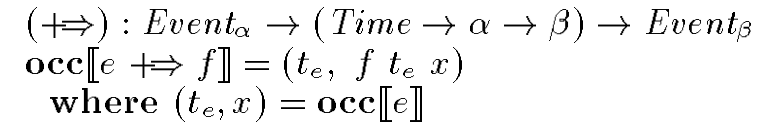
\includegraphics[scale=0.75]{pics/1.png}
	\label{pic:1}
\end{figure}

	Patogumui galima naudoti šias išvestas operacijas, kurios ignoruoja laiką arba informaciją arba abu kartu:

\begin{figure}[H]
	\centering
	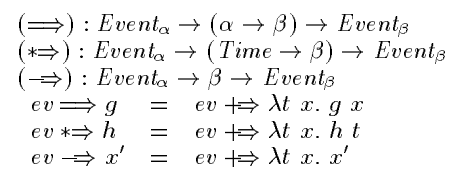
\includegraphics[scale=0.75]{pics/2.png}
	\label{pic:2}
\end{figure}

	(+$\Rightarrow$) gauna visus parametrus, (-$\Rightarrow$)  negauna parametrų, (*$\Rightarrow$) gauna tik laiką, o ($\Longrightarrow$) gauna tik informaciją.

	\item \textbf{Nekintantys įvykiai}. Paprasčiausia įvykių rūšis yra tiesiogiai specifikuoti pagal laiką ir reikšmę.

\begin{figure}[H]
	\centering
	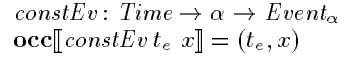
\includegraphics[scale=0.75]{pics/3.png}
	\label{pic:3}
\end{figure}

	Nors, pavyzdžiui, elgesys:

\begin{figure}[H]
	\centering
	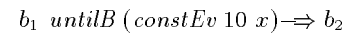
\includegraphics[scale=0.75]{pics/4.png}
	\label{pic:4}
\end{figure}

	parodo elgesį \(b_{1}\) iki laiko taško 10, kuriame jis pradeda rodyti elgesį \(b_{2}\) (x yra ignoruojamas šiame pavyzdyje, bet iš tikro neturėtų).

	\item \textbf{Išoriniai įvykiai}. Išoriniai įvykiai yra pavyzdžiui pelės mygtuko paspaudimas, kuris gali būti kairysis arba dešinysis mygtukas. Reikšmė, asocijuota su kurio nors mygtuko paspaudimu yra interpretuojama kaip atleidimo įvykis, kuris grąžina vienetinę reikšmę (() yra vieneto tipas):

\begin{figure}[H]
	\centering
	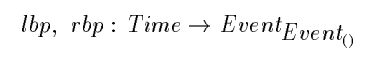
\includegraphics[scale=0.75]{pics/5.png}
	\label{pic:5}
\end{figure}

	Įvykio \textit{lbp \(t_{0}\)} prasmė, pavyzdžiui, yra pora (\(t_{e}\), e), tokia kad \(t_{e}\) yra pirmojo kairio mygtuko paspaudimas po laiko \(t_{0}\) ir \textit{e} yra įvykis, reiškiantis pirmojo kairiojo mygtuko atleidimą po laiko \(t_{e}\). Iš to seka, jog:

\begin{figure}[H]
	\centering
	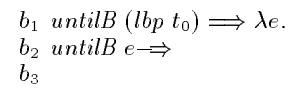
\includegraphics[scale=0.75]{pics/6.png}
	\label{pic:6}
\end{figure}

	parodo elgesį \(b_{1}\) iki kairiojo mygtuko paspaudimo, kurio metu jis tampa \(b_{2}\) kol kairysis mygtukas yra atleistas, o tada tampa \(t_{3}\).

	\item \textbf{Predikatai}. Natūralus būdas specifikuoti tam tikrus įvykius kaip pirmąjį laiką kada loginės reikšmės elgesys tampa tiesa (\textit{true}) po duoto laiko:

\begin{figure}[H]
	\centering
	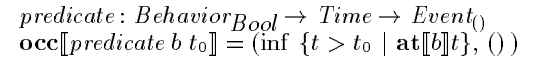
\includegraphics[scale=0.75]{pics/7.png}
	\label{pic:7}
\end{figure}

	Predikato įvykio laikas yra begalinis ir sudarytas iš rinkinio laiko taškų didesnių tei \(t_{0}\), kuriuose elgesys yra teigiamas. Šis laikas gali būti ir \(t_{0}\).

	Tada elgesys:

\begin{figure}[H]
	\centering
	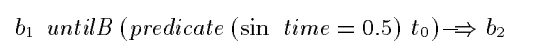
\includegraphics[scale=0.75]{pics/8.png}
	\label{pic:8}
\end{figure}

 	parodo \(b_{1}\) iki pirmojo laiko taško t po \(t_{0}\), kur \textit{sin t} yra 0.5, po kurio jis parodo \(b_{2}\).

 	\item \textbf{Pasirinkimas}. Galima pasirinkti ankstesnįjį iš dviejų įvykių naudojantis operatoriumi .|.:

\begin{figure}[H]
	\centering
	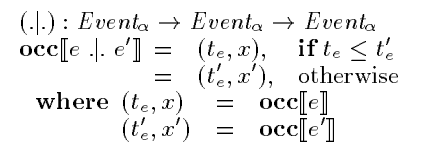
\includegraphics[scale=0.75]{pics/9.png}
	\label{pic:9}
\end{figure}

	Pavyzdžiui, elgesys:

\begin{figure}[H]
	\centering
	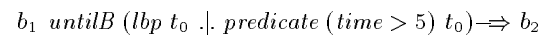
\includegraphics[scale=0.75]{pics/10.png}
	\label{pic:10}
\end{figure}

	laukia kol arba bus nuspaustas kairysis mygukas arba praeis 5 sekundės prieš pakeičiant \(b_{1}\) elgesį į \(b_{2}\). Kaip alternatyva, sekantis pavyzdys pakeičia elgesį į \(b_{3}\) po skirto laiko pabaigos:

\begin{figure}[H]
	\centering
	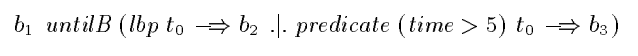
\includegraphics[scale=0.75]{pics/11.png}
	\label{pic:11}
\end{figure}

	\item \textbf{Momentinė kopija}. Tuo momentu kai nutinka įvykis yra dažnai patogu padaryti elgesio reikšmės momentinę kopiją tam tikrame laiko taške. Tai formaliai galima užrašyti:

\begin{figure}[H]
	\centering
	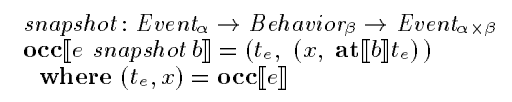
\includegraphics[scale=0.75]{pics/12.png}
	\label{pic:12}
\end{figure}

	Pavyzdžiui, elgesys:

\begin{figure}[H]
	\centering
	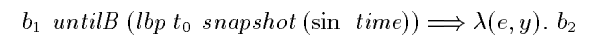
\includegraphics[scale=0.75]{pics/13.png}
	\label{pic:13}
\end{figure}

	paima laiko, kai yra nuspaudžiamas kairysis mygtukas, sinusą, priskiria jį \textit{y} ir seka elgesiu \(b_{2}\), kuris galimai priklauso nuo \textit{y}. Nepaisant to, šį pavyzdį taip pat būtų galima realizuoti paimant kairiojo mygtuko paspaudimo įvykio laiką ir skaičiuojant sinusą, bendru atveju elgesio buvimas momentine kopija yra ganėtinai sudėtingas ir gali priklausyti nuo išorinių įvykių.

	\item \textbf{Įvykių sekos} Kartais yra naudinga naudoti vieną įvykį, kad būtų galima sukurti kitą. Įvykis \textit{joinEv e} yra įvykio, kuris nutinka kai nutinka \textit{e'}, kur \textit{e'} yra \textit{e} reikšmės dalis:

\begin{figure}[H]
	\centering
	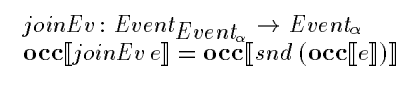
\includegraphics[scale=0.75]{pics/14.png}
	\label{pic:14}
\end{figure}

	Pavyzdžiui, įvykis:

\begin{figure}[H]
	\centering
	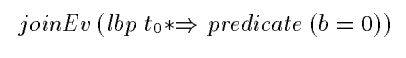
\includegraphics[scale=0.75]{pics/15.png}
	\label{pic:15}
\end{figure}

	nutinka pirmą kartą kai elgesys \textit{b} turi nulinę reikšmę po pirmojo kairiojo mygtuko paspaudimo po laiko tarpo \(t_{0}\).

\end{itemize}

\textbf{Panaudojimo pavyzdys}

Remiantis primityvių kombinatorių pavyzdžiais elgesiui bei įvykiam kartu su jų formalia semantika, galima pateikti konkretų pavyzdį Haskell programavimo kalboje. \ref{sign} pateiktame pavyzdyje yra skaitine reikšme išreikštas elgesys, kurio pradinė reikšmė yra 0 ir tampa -1 jeigu yra nuspaustas kairys pelės mygtukas arba 1 jeigu yra nuspaustas dešinys pelės mygtukas.

\begin{lstlisting}[caption=- signalo funkcija nuo pelės mygtuko paspaudimo, label=sign]
	bSign t0 =
		0 'untilB' lbp t0 ==> nonZero (-1) .|.
				   rbp t0 ==> nonZero 1
		where nonZero r stop =
				r 'untilB' stop *=> bSign
\end{lstlisting}

Šį elgesį galima panaudoti paveikslėlio dydžio keitimui. Kairio arba dešinio pelės mygtuko paspaudimas priverčia paveikslėlį padidėti arba sumažėti. Pavyzdys pateiktas \ref{grow}.


\begin{lstlisting}[caption=- paveiksliuko dydžio modifikavimas pelės paspaudimu, label=grow]
	bSign t0 =
		0 'untilB' lbp t0 ==> nonZero (-1) .|.
				   rbp t0 ==> nonZero 1
		where nonZero r stop =
				r 'untilB' stop *=> bSign
\end{lstlisting}



%%%%%%%%%%%%END SEMANTIKA

\subsubsection{Įvykių srautas}

Pagal \cite{Bass:2007:Mythbusters}, įvykių srautas yra eilė pagal laiką surikiuotų įvykių, pavyzdžiui akcijų rinkos srautas.

Įvykių srautas kaip duomenų srauto tipas formaliai atrodo kaip pora (s, t), kur s yra seka surikiuotų sąrašo įvykių, o t yra seka laiko intervalų ir kiekvienas intervalas yra netuščias.

Tokio duomenų srauto pavyzdžiai gali būti:

\begin{itemize}

	\item akcijų kursas,

	\item paspaudimų srautas,

	\item tinklo srautas,

	\item GPS duomenys.

\end{itemize}

Įvykių srauto apdorojimas pagal atsitikimo laiką turi privalumų:

\begin{itemize}

	\item įvykių apdorojimo algoritmai naudoja mažai atminties, nes jiems nereikia prisiminti daug įvykių;

	\item algoritmai gali būti labai greiti;

	\item gavus įvykį, skaičiavimai atliekami iškart, todėl galima perduoti rezultatą kitam skaičiavimui ir pamiršti įvykį.

\end{itemize}

Įvykių srauto apdorojimas labiau akcentuoja didelio našumo duomenų gavimą ir matematinių algoritmų pritaikymą įvykių duomenims. Taip pat įvykių srautai įprastai pritaikomi konkrečiai sistemai ar organizacijai.
